\documentclass{report}

\usepackage[francais]{babel}
\usepackage[utf8x]{inputenc}
\usepackage[T1]{fontenc}
\usepackage[final]{pdfpages}
\usepackage{graphicx}
\usepackage{array}
\usepackage{eurosym}
\usepackage{listings}

\title{Université de Technologie Belfort-Montbéliard\\
Projet LO41\\
Centre d'appels}
\author{Guillaume OBERLE\\
Alexandre THIERIOT}

\lstdefinestyle{customc}{
  belowcaptionskip=1\baselineskip,
  xleftmargin=\parindent,
  language=C,
  showstringspaces=false,
  basicstyle=\footnotesize\ttfamily,
  keywordstyle=\bfseries\color{green!35!black},
  commentstyle=\itshape\color{purple!30!black},
  identifierstyle=\color{blue},
  stringstyle=\color{orange},
}

\lstset{escapechar=@,style=customc}

\begin{document}

\makeatletter
\def\clap#1{\hbox to 0pt{\hss #1\hss}}%
\def\ligne#1{%
\hbox to \hsize{%
\vbox{\centering #1}}}%
\def\haut#1#2#3{%
\hbox to \hsize{%
\rlap{\vtop{\raggedright #1}}%
\hss
\clap{\vtop{\centering #2}}%
\hss
\llap{\vtop{\raggedleft #3}}}}%
\def\bas#1#2#3{%
\hbox to \hsize{%
\rlap{\vbox{\raggedright #1}}%
\hss
\clap{\vbox{\centering #2}}%
\hss
\llap{\vbox{\raggedleft #3}}}}%

\def\maketitle{%
\thispagestyle{empty}\vbox to \vsize{%
\haut{}{\@blurb}{}
\vfill
\vspace{1cm}
\begin{flushleft}
\usefont{OT1}{ptm}{m}{n}
\huge \@title
\end{flushleft}
\hrule height 4pt
\begin{flushright}
\usefont{OT1}{phv}{m}{n}
\large \@author
\end{flushright}
\begin{flushleft}
\end{flushleft}
\vspace{1cm}
\vfill
\begin{center}

\includegraphics[width=.5\textwidth]{./logo.png}
\end{center}
\vfill
\vfill
\bas{}{\@location, le \@date}{}
}%
\cleardoublepage
}
\def\date#1{\def\@date{#1}}
\def\author#1{\def\@author{#1}}
\def\title#1{\def\@title{#1}}
\def\location#1{\def\@location{#1}}
\def\blurb#1{\def\@blurb{#1}}
\makeatother

\title{Centre d'appel\\ \large Rapport de projet}
\author{Alexandre \textsc{Thieriot} \\ Guillaume \textsc{Oberle}}
\location{Belfort}
\blurb{%
Rapport de projet de LO41\\
Université de Technologie de Belfort-Montbeliard
}

\maketitle

\tableofcontents

\chapter{Introduction}
	\paragraph{}
		Dans le cadre de l'UV LO41 : Architecture et utilisation des systèmes d'exploitation, nous avons travaillé sur la conception d'un projet qui a pour objectif de simuler un centre d'appel téléphonique. Les connaissances acquises depuis le début de cette UV nous ont permi de concevoir cette simulation avec la programmation système.
	\paragraph{}
		Un centre d'appel est un ensemble de moyens, humains, immobiliers, mobiliers et techniques, qui permet de prendre en charge la relation à distance entre une marque et son marché. Dans le cadre ce projet, nous n'étudierons que l'aspect technique de la mise en place d'un centre d'appel, et plus précisement le fonctionnement de la mise en relation d'un client avec un agent.
	\paragraph{}
		Le développement de notre rapport sera divisé en trois parties. Dans un premier temps, nous présenterons le cahier des charges. Puis dans un second temps, notre présenterons les différents programmes qui composent notre projet. Et enfin, dans un dernier temps, nous expliquerons comment ces différents programmes intéragissent entre eux.

\chapter{Cahier des charges}
	\paragraph{}
	L'énoncé du problème est le suivant:
	\paragraph{}
		Ce projet doit être réalisé en C sous environnement OpenSolaris. Un centre d'appels a pour fonction de répondre aux demandes d'informations du public. Pour se faire, un numéro est donc mis à disposition du public et plusieurs opérateurs ont la charge de traiter les appels. Trois cas de figures peuvent se présenter :
	\paragraph{}
		\begin{itemize}
			\item Il y a au moins un opérateur disponible. L'appel va donc être traité immédiatement.
			\item Il n'y a pas d'opérateur de libre, mais on estime que l'attente prévisible est acceptable. On va donc faire patienter le client jusqu'à ce que l’opérateur se libère.
			\item Il n'y a pas d’opérateur de libre et on estime que l'attente prévisible n'est pas acceptable. On va donc dissuader l'appel. Le client sera informé par un message vocal que son appel ne peut pas être traité et il sera donc invité à rappeler ultérieurement.
		\end{itemize}
	\paragraph{}
		Nous considérons un pilote comme étant l'entité qui gère un numéro de téléphone unique. Cette entité servira à placer un appel qu'il reçoit dans une file d'attente avant qu'un opérateur prenne en charge l'appel. Un groupe de traitement rassemble plusieurs opérateurs que nous appelerons agents. Un groupe de traitement appartient à un service. Il prendra en priorité les appels destinés à son service (c'est à dire les appels chez un pilote spécifique) mais pourra également s'occuper des appels appartenant à un service autre que le sien si celui-ci ne reçoit plus d'appel sur son service.
	\paragraph{}
		Prenons par exemple un agent appartenant au service commercial d'une entreprise. Le service commercial peut également s'occuper des appels destinés au service résiliation (ce service fait en effet également appel à des compétences commerciales). C'est pourquoi lorsque cet agent ne recevra plus d'appel à son service initial, celui-ci pourra aider les agents du service résiliation en leur prennant quelques appels. Lorsque de nouveaux appels destinés au service commercial referont surface, cet agent pourra reprendre ces appels.
	\paragraph{}
		Le nombre de groupes de traitement et de pilotes sera de 64 par défaut mais l'utilisateur pourra également abaisser ce nombre. L'attente d'un appel devra se faire selon le principe "FIFO", c'est à dire que le premier appel arrivant sera le premier pris en charge par les agents.

\chapter{Présentation des acteurs}
	\section{Programme central}
		\paragraph{}
			Le central a pour objectif de créer et gérer tous les IPCs relatifs au bon fonctionnement des pilotes ainsi que des groupes de traitements. Il va notamment créer un segment de mémoire partagée ainsi que les files de messages utilisées pour la communication inter processus. Le programme permet également de consulter durant son exécution, l'état et le nombre de messages dans la file d'attente ainsi que dans la file de dissuasion. Enfin, il permet de la supprimer lorsque l'utilisateur le souhaite.

	\section{Programme pilote}
		\subsection{Présentation des pilotes}
			Le pilote permet de générer à des temps alétoires un appel. Ceci fait référence au fait qu'un appel peut être reçu à un temps incertain. Un appel est caractérisé par le nom de l'appelant, défini comme étant la composition du numéro du pilote et du nombre de messages déjà générés par ce pilote (utilisé à des fin de vérification au bon fonctionnement du programme), le numéro sur lequel celui-ci a appelé (qui se situe entre le numéro +334 50 29 00 et le numéro +334 50 29 63 symbolisant la plage de numéros réservés par l'entreprise) et la durée de son appel, généré aléatoirement. Cet appel est placé dans une file d'attente que nous détaillerons dans les parties suivantes.
		\subsection{Fonctionnement d'un pilote}
			Un pilote est considéré comme étant un thread. Tous les pilotes créés sont répertoriés dans un tableau de type pthread\_t de taille nbPilote, le nombre de pilotes que l'on souhaite créer. Chaque thread est exécuté avec la fonction threadPilote.

	\section{Programme groupe de traitement (GT)}
		\subsection{Présentation d'un groupe de traitement}
			Un groupe de traitement est composé d'un ou plusieurs agents dans une limite de 64 agents maximum. Son rôle est de récupérer les appels qui lui correspondent en file d'attente et de les attribuer aux agents disponibles lui appartenant. Pour ce faire, nous avons utilisé l'algorithme du producteur-consommateur vu en cours. Le GT jouant le rôle du producteur et les agents jouant le rôle des consommateurs.
		\subsection{Fonctionnement d'un groupe de traitement}
			Un groupe de traitement est un thread. Ce thread est exécuté grâce à la fonction threadGt. Aprés sa création, celui-ci va s'occuper de créer les threads agents qui lui sont associés et va mettre en oeuvre l'algorithme du producteur-consommateur.
			\paragraph{Le mutex}
				Pour mettre en oeuvre l'algorithme du producteur consommateur nous avons eu recours à l'utilisation de mutex. En effet, chaque GT possède un mutex afin que les différents entitées (producteur et consommateurs) souhaitant avoir accès au tampon ainsi qu'au nombre de messages actuellement dans le tampon soit en exclusion mutuelle. 
			\paragraph{Les moniteurs}
				Nous avons également utilisé les moniteurs pour gérer la synchronisation du tampon. Deux sont nécessaires pour mettre en oeuvre cette synchronisation : l'un pour avertir qu'une place dans le tampon est libre et l'autre pour avertir qu'un message a été ajouté dans le tampon. 
		\subsection{Structure d'un groupe de traitement}
			\paragraph{}
				Voici la structure d'un groupe de traitement.
			\paragraph{}
				\lstset{language=C}
				\begin{lstlisting}
typedef struct Gt_t {
	pthread_t thread; 		/* ID du thread d'un GT */
	int msqid;			/* ID de la file d'attente a traiter */
	int nbFiles;	 		/* Nombre de types de files */
	int noFiles[NB_FILE]; 		/* Types de files a traiter */
	int nbAgents; 			/* Nombre d'agents appartenant au GT */
	agent_t agent[NB_AGENT]; 	/* Agents appartenant au GT */
	pthread_mutex_t mutex; 		/* Mutex */
	pthread_cond_t nonPlein; 	/* Condition 1 */
	pthread_cond_t nonVide; 	/* Condition 2 */
	int idProd; 			/* Indice du producteur */
	int idCons; 			/* Indice du consommateur */
	int nbMsg;			/* Nombre de messages dans le tampon */
	int sizeTampon; 		/* Taille du tampon */
	msq_t msqTampon[SIZE_TAMPON]; 	/* Tampon */
} gt_t;
				\end{lstlisting}
		\subsection{Fonctionnement d'un agent}
			L'agent est un thread qui est créé par le groupe de traitement auquel il appartient. Ce thread est exécuté grâce à la fonction threadAgent. Il joue le rôle du consommateur et possède ainsi deux états : soit il est en attente d'un message, soit il est en train de traiter un message.
		\subsection{Structure d'un agent}
			\paragraph{}
				Voici la structure d'un agent.
			\paragraph{}
				\lstset{language=C}
				\begin{lstlisting}
typedef struct {
	int id;			/* ID de l'agent */
	pthread_t thread;	/* Identifiant du thread d'un agent */
	struct Gt_t* gt;	/* GT dans lequel se situe l'agent */
} agent_t;
				\end{lstlisting}
	\newpage
	\section{Réseau de Pétri}
		\paragraph{}
			\begin{center}
				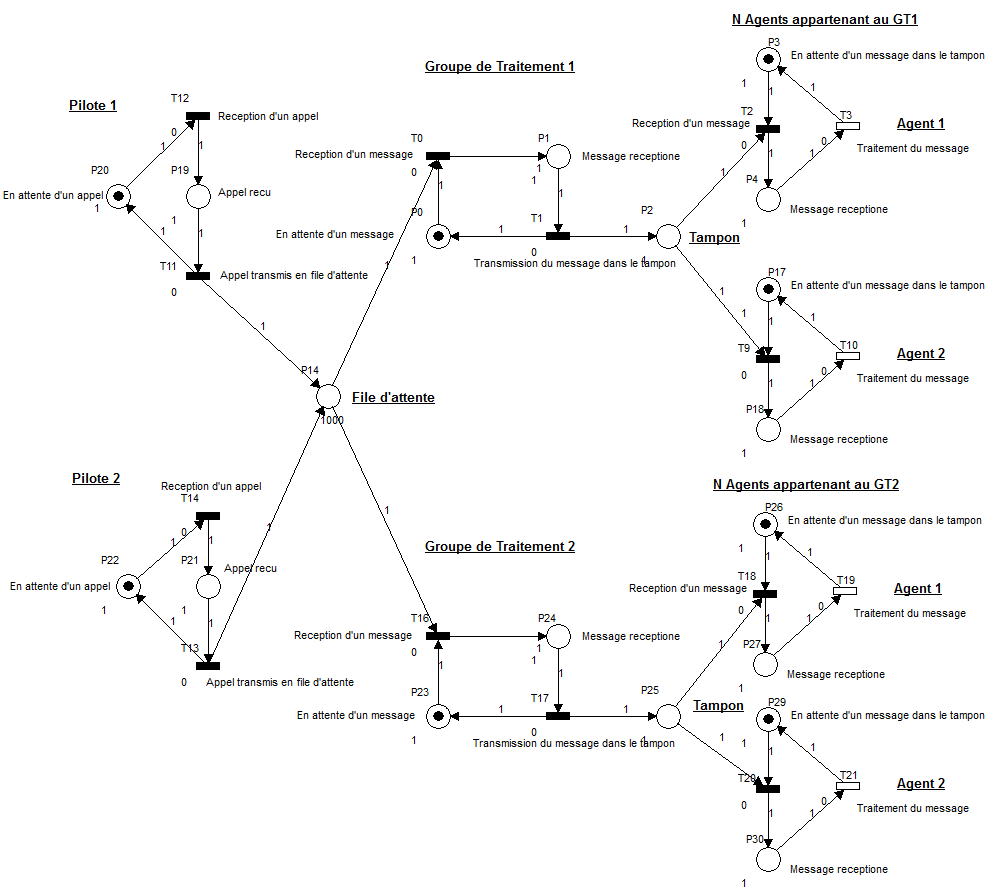
\includegraphics[scale=0.50]{petri.png}
			\end{center}
\chapter{Communication inter processus}
	\section{La mémoire partagée}
		\paragraph{}
			La mémoire partagée permet de stocker toutes les informations relatives aux groupes de traitements, et notamment les types de files d'attentes qu'ils peuvent traiter. Cette mémoire partagée est utilisée dans le pilote pour rechercher un groupe de traitement disponible et apte à traiter ce type d'appel.

		\subsection{Groupe de traitement}
			Lors du lancement du processus des groupes de traitement, celui-ci va parser un fichier de configuration qui contient pour chaque GT, le nombre d'agents ainsi que leur file par défaut et leurs files de débordement. Celà permet de configurer à souhait chaque groupe de traitement.

		\subsection{Pilote}
			Lorsqu'un appel arrive sur un pilote, celui-ci va parcourir les groupes de traitements, via la mémoire partagée, à la recherche d'un qui correspond à son type d'appel. Il cherchera en priorité à savoir si le GT par défaut pour son type d'appel est susceptible de traiter l'appel. Sinon, il partira à la recherche d'un GT de débordement disponible. Si aucun GT n'est disponible, il placera l'appel dans le GT par défaut. Pour connaitre la disponibilité d'un GT, le pilote cherchera à savoir si le tampon du GT donné (lié à l'algorithme du producteur-consommateur) est plein ou non. Une fois le choix du GT effectué, celui-ci va typer l'appel (le message) pour que le bon GT puisse récupérer le message en file d'attente.

	\section{Les files de messages}
		\paragraph{}
			Afin de gérer le traitement des appels, l'utilisation des files de message correspondait parfaitement au cahier des charges. Tout d'abord, le fonctionnement en FIFO de la file de message, c'est à dire du "premier arrivé, premier servi" permet à la file de message d'être utilisée en tant que file d'attente. De plus la file de message nous permet de gérer très facilement la redirection des appels vers la file de dissuasion. En effet, pour ajouter un appel dans la file d'attente, si la file de message principale (la file d'attente) est pleine, l'appel sera donc redirigé vers la file de dissuasion. Le fonctionnement de la file de dissuasion fonctionne de la même manière que la file d'attente. Lorsque les deux files sont pleines, l'appel sera rejeté. La file de message a de plus l'avantage de gérer par défaut le typage des messages ainsi que les problèmes d'accès concurrentiels.
		\paragraph{Le pilote}
			Une fois le typage de l'appel réalisé grâce au segment de mémoire partagée, le pilote dépose l'appel soit en file d'attente, soit en file de dissuasion selon la disponibilité de chacune. Si les deux sont pleines, l'appel ne sera pas traité.
		\paragraph{Groupe de traitement}
			Chaque groupe de traitement cherche un message de son type en file d'attente pour le mettre dans son tampon. S'il ne trouve pas de message de son type, il reste bloqué jusqu'à ce qu'un message de son type est envoyé dans la file de message.

\chapter{Conclusion}
	\section{Problèmes rencontrés}
		\paragraph{}
			Il ne nous a pas été possible de créer au moins 64 agents par GT. En effet, le système d'exploitation est limité à un certain nombre de thread par processus. C'est pourquoi nous avons choisi de conserver les 64 GT mais nous avons été contraint de réduire le nombre d'agent par GT de 64 à environ 32.
		\paragraph{}
			Nous nous étions fixé au début de la conception du projet que les pilotes avaient pour seule fonction d'envoyer des messages dans la file de message en ne se souciant pas des priorités. C'est à dire par exemple que le pilote 32 envoyait des messages de type 32 à destination du GT 32. C'était ensuite le scheduler du GT32 qui devait s'occuper de gérer les priorités. C'est à dire que celui-ci avait pour objectif de vérifier dans la file de message, s'il existait un message de son type (c'est à dire de type 32). Si celui-ci ne trouvait aucun message à récupérer, il passait alors sur la première priorité de débordement. S'il n'y avait pas de message présent dans cette file de débordement, il passait ensuite à la file de débordement suivante, etc. Lorsque un nouveau message arrivait dans sa priorité principal, le scheduler revenait à cette première priorité pour traiter ce message. Le problème était que s'il n'existait jamais de message présent dans les files de débordement qu'il parcourait, la recherche était comparable à une attente active puisque le scheduler cherchait sans cesse dans chacune de ses priorités. 
		\paragraph{}
			L'ajout du stockage des groupes de traitement dans un segment de mémoire partagé ainsi que la recherche pour l'assignation des appels par les pilotes nous ont permis de palier ce problème.

	\section{Compilation et exécution du programme}
		\paragraph{Compilation}
			La compilation du programme s'effectue via un Makefile. Trois cibles sont importantes :
			\begin{itemize}
				\item make mrproper : permet de supprimer les fichiers executables ainsi que les fichier objets
				\item make clean : permet de supprimer les fichiers objets
				\item make all : permet de réaliser la compilation des programmes
			\end{itemize}

		\paragraph{Execution}
			Afin d'exécuter le programme, nous avons mis à disposition plusieurs fichiers de configuration (gt\_config, gt\_config1, gt\_config2, gt\_config3). Chaque ligne d'un fichier de configuration correspond à la configuration d'un GT. Cela permet donc de définir les options de lancement de chaque groupe de traitement. Une ligne est définie de la manière suivante : [Nombre d'agents à créer dans le GT], [Numero du GT], [File de débordement 1], [File de débordement 2], [File de débordement 3], [File de débordement 4], [File de débordement 5].
		\paragraph{}
			Afin d'assurer le bon fonctionnement du programme, l'utilisateur doit obligatoirement lancer le même nombre de pilotes que de groupe de traitement et il doit suivres ces étapes :
			\begin{enumerate}
				\item Exécution du programme central : ./central
				\item Exécution des groupes de traitements : ./gt [N Nombre de GT à lancer] [Nom du fichier de configuration]
				\item Exécution des pilotes : ./pilote [N Nombre de pilotes à lancer] [Attente minimum d'un pilote après la transmission d'un appel] [Attente maximum d'un pilote après transmission d'un appel] [Durée minimum d'un appel] [Durée maximum d'un appel]
			\end{enumerate}

	\section{Conclusion finale}
		\paragraph{}
			Pour finir, nous avons trouvé ce sujet intéressant car il nous a permis de mettre en oeuvre les notions que nous avons abordé en cours dans le cadre d'une simulation pouvant donner suite à une utilisation grandeur nature. De plus nous avons réfléchi à d'autres fonctionalités que nous pourrions ajouter tel que la possibilité d'ajouter et de supprimer des agents dans un groupe de traitement. Cependant le manque de temps ne nous a pas permis de le finaliser. Enfin, ce projet nous a également permis de nous entrainer sur les problèmes de synchronisation et de communication entre processus. 

\chapter{Annexe}
	\section{Présentation de la bibliothèque libmsq}
		\paragraph{}
			La bibliothèque libmsq contient toutes les fonctions utiles à la gestion d'une file de message et aux contrôles des erreurs.
			\begin{itemize}
				\item createMsq est la fonction qui permet de créer la file de message. Elle prend en paramètre un entier et retourne l'identifiant de la file de message ou -1 si l'appel à la fonction msgget n'a pas marché. La fonction fait appel à la fonction msgget paramètré avec le drapeau IPC\_CREAT.
				\item deleteMsq est la fonction qui permet de supprimer une file de message. Elle prend en paramètre l'identifiant de la file de message et renvoie 1 si la suppression a fonctionné, -1 sinon. La fonction fait appel à la fonction msgctl paramètrée avec le drapeau IPC\_RMID.
				\item connectMsq est la fonction qui permet à un processus ou un thread de se connecter à une file de message existante. Elle prend en paramètre un entier et renvoie le numéro de la file de message correspondante.La fonction fait appel à la fonction msgget paramètrée avec le drapeau IPC\_EXCL.
				\item sendMsq est la fonction qui permet d'envoyer un message vers la file de message. Elle renvoie 1 si l'envoi a marché, -1 sinon. La fonction fait appel à la fonction msgsnd paramètrée avec le drapeau IPC\_NO\_WAIT. Ce drapeau permet à msgsnd ne pas rester bloquer si la file de messag est pleine( en effet par défaut, msgsnd attendra qu'une place dans la file de mesage se libère ). Si la file de message est pleine, msgsnd renverra -1 et errno sera égal à EAGAIN.
				\item rcvMsq est la fonction utilisée pour récupérer un message situé dans la file de message. Elle renvoie 1 si la récupération a fonctionné et est bloqué si la file de message est vide. Elle envoie un message d'erreur si l'envoie a échoué. La fonction fait appel à la fonction msgrcv qui est bloquante si la file de message est vide.
			\end{itemize}
	\section{Présentation de la bibliothèque libshm}
			\paragraph{}
				La bibliothèque libshm contient toutes les fonctions utiles à la gestion du segment de mémoire partagée.
				\begin{itemize}
					\item createShm est la fonction qui permet de créer un segment de mémoire partagée. Elle renvoie l'identifiant du segment si la création a réussi, -1 sinon. La fonction fait appel à la fonction shmget avec le drapeau IPC\_CREAT afin de créer le segment.
					\item deleteShm est la fcontion qui permet de supprimer un segment de mémoire partagée. La fonction renvoie 1 si la suppression a fonctionné, -1 sinon. Celle-ci utilise la fonction shmctl avec le drapeau IPC\_RMID afin du supprimer le segment.
					\item connectShm est la fonction qui permet à un processus de connaitre l'identifiant d'un segment de mémoire partagée déjà créé. Elle renvoie l'identifiant du segment si celle-ci a réussi, -1 sinon. La fonction fait appel à la fonction shmget associée au drapeau IP\_EXECL.
				\end{itemize}

\end{document}
